\documentclass[a4paper]{book}

\usepackage[margin=1.5cm]{geometry}
\setlength{\parindent}{0cm} 
\usepackage[utf8]{inputenc}
\usepackage[T1]{fontenc}

\usepackage{polyglossia}
  \setmainlanguage{german}

\usepackage{fontspec}
  \setmainfont{EB Garamond}

\usepackage[german=guillemets]{csquotes}
\usepackage[hidelinks]{hyperref}

\usepackage{multicol}
  \setlength{\columnsep}{1cm}

\usepackage{graphicx}
\usepackage{needspace}
% format section, subsection and subsubsection headings
\newcounter{mysubsection}[section]
\newcounter{mysubsubsection}[mysubsection]

\usepackage{titlesec}
  \titleformat{\section}{\LARGE\scshape\filcenter}{}{1em}{}
  \titleformat{\subsection}{\Large\scshape\filcenter}{\stepcounter{mysubsection} \themysubsection
}{1em}{}
  \titleformat{\subsubsection}{\Large\filcenter}{\stepcounter{mysubsubsection}\themysubsection . \themysubsubsection}{1em}{}

\pagenumbering{roman}

% provide number of last page to be used by fancyhdr 
\usepackage{zref-abspage,zref-lastpage}
\makeatletter
\newcommand*{\iffancylastpage}{%
    \ifnum\zref@extractdefault{LastPage}{abspage}{-1}%
        =\numexpr\value{abspage}+1\relax
      \expandafter\@firstoftwo
    \else
      \expandafter\@secondoftwo
    \fi
  }
\makeatother
\usepackage{fancyhdr}
  \pagestyle{fancy}
  \fancyhf{} % clear header and footer
  \renewcommand{\headrulewidth}{0pt}  % remove headrule
  \fancyhead[LO, RE]{\thepage}  % book-like pagenumbering in header
  
  \fancyfoot[R]{  % Version on last page
    \iffancylastpage{Revision Nr. 1.0.1 | 11. Juni 2022}{}%
  }

% necessary for having footnote in caption
\usepackage{ftnxtra}

% necessary things for the interlinear translation
\usepackage{stackengine}
  \setstackEOL{\cr}

\begin{document}

\section{Editorische Anmerkungen}

\subsection{Quelle}

Quelle der vorliegenden Edition ist das Autograph,\footnote{Musiksammlung der Österreichischen Nationalbibliothek, Wien (W) Mus.Hs.44018} das Bruckner am 3.9.1885 anfertigte, in seiner digitalisierten Form von bruckner-online.at \footnote{\url{http://www.bruckner-online.at/?page_id=1588}, \url{http://www.bruckner-online.at/mirador.php?Signatur=A-WnMus.Hs.44018}}

\begin{figure}[h]
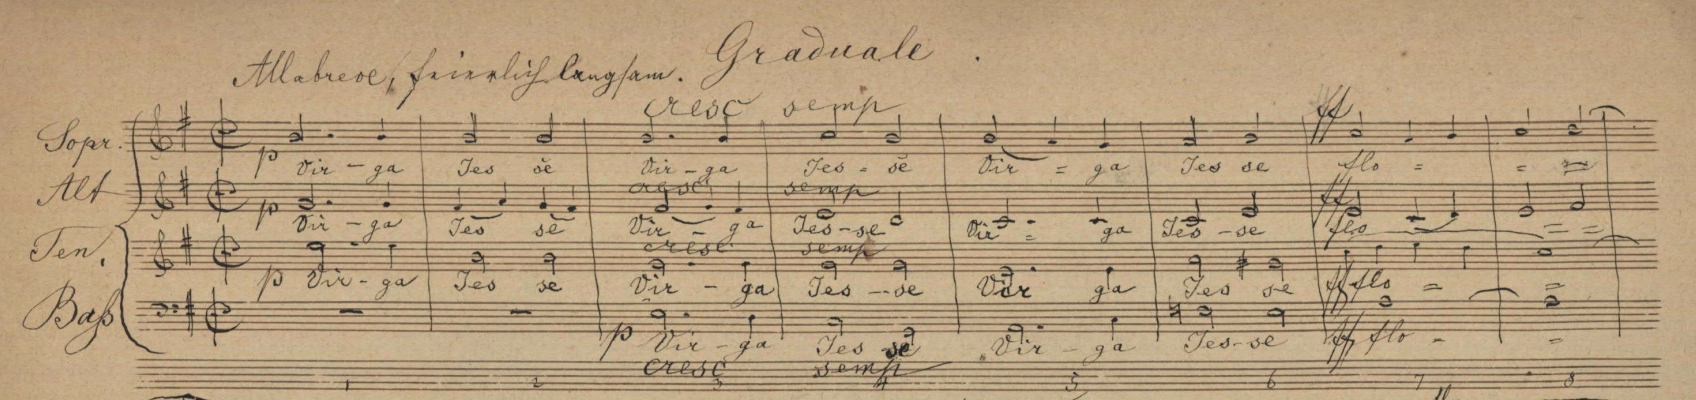
\includegraphics[width=\textwidth]{Graduale_First_System.png}
\caption{Das erste System aus dem Autograph von \emph{Virga Jesse}}
\end{figure}

\section{Kommentar zum Text}

\subsection{Interlinearübersetzung}

\begin{center}
\input{translation.iltex}
\end{center}

\subsubsection{Abkürzungen}
\begin{multicols}{4}
  \noindent Abl.: \textit{Ablativ} \\
  Akk.: \textit{Akkusativ} \\
  Akt.: \textit{Aktiv} \\
  Dat.: \textit{Dativ} \\
  Ind.: \textit{Indikativ} \\
  Nom.: \textit{Nominativ} \\
  Part.: \textit{Partizip} \\
  Perf.: \textit{Perfekt} \\
  Pers.: \textit{Person} \\
  Präs.: \textit{Präsens} \\
  Sgl.: \textit{Singular} \\
\end{multicols} 

\pagebreak

\begin{samepage}

\Needspace{6\baselineskip}
\subsection{Aspekte der Interpretation}

\begin{multicols}{2}

Der Text behandelt, wie auch andere bekannte Weihnachtslieder,\footnote{etwa \emph{Es ist ein Reis entsprungen}, \emph{Wie schön leuchtet der Morgenstern}} die christliche Vorstellung, dass sich in der Geburt Jesu durch die Jungfrau Maria die alttestamentarische Prophezeihung des Messias aus dem Buch Jesaja erfüllt: 

\begin{quote}
Jesaja 11,1: VND es wird eine Rute auffgehen von dem stam Jsai [Jesse] / vnd ein Zweig aus seiner wurtzel Frucht bringen.\footnote{Bibelübersetzung von Martin Luther, 1545, zit. n. \url{https://www.bibel-online.net/buch/luther_1545_letzte_hand/jesaja/11/\#1}}

Jesaja 7, 14: Darumb so wird euch der HErr selbs ein Zeichen geben / Sihe / Eine Jungfraw ist schwanger / vnd wird einen Son geberen / den wird sie heissen Jmmanuel.\footnote{ebd., zit. n. \url{https://www.bibel-online.net/buch/luther_1545_letzte_hand/jesaja/7/\#14}}
\end{quote}

Diese Bezugnahme auf die Prophezeiung Jesajas im Alten Testament und auf die Abkunft Jesu von Jesse, den Vater König Davids, ist für die christliche Vorstellung von der Messiashaftigkeit Jesu von Bedeutung. Im Matthäus- und im Lukas-Evangelium wird die Abkunft Jesu bis auf Abraham, bzw. bis auf Adam zurückgeführt, in beiden Stammlinien tauchen auch David und Jesse auf. Ziel dieser Abstammungsangaben ist es, Jesus in die biblische Heilsgeschichte Israels einzuordnen. 

Der Stammbaum Jesu bis hinauf zu Jesse ist auch Gegenstand zahlreicher bildlicher Darstellungen, die vom Mittelalter über die Renaissance bis in die Moderne reichen.

Der Text betont den Zusammenhang zwischen der Geburt Jesu und der Prophetie Jesajas auch mit formensprachlichen Mitteln: indem die beiden ersten Verse grammatisch parallel geführt sind, und auch durch das Spiel mit der Klangähnlichkeit von VIRGA (\enquote{der Zweig}) und VIRGO (\enquote{die Jungfrau}), wird eine identifzierende Analogie von Maria mit der Wurzel Jesse nahegelegt. Diese Analogie wird weiter unterstützt durch den Allegorienkomplex der aus dem Zweig Jesse erblühenden Blüte, die in einer konventionellen Metapher für die Jungfräulichkeit, hier für diejenige Marias, steht.\footnote{Dieser Allegorienkomplex wird etwa auch im Weihnachtslied \emph{Es ist ein Ros entsprungen} verwendet.}

\end{multicols}

\end{samepage}

\begin{figure}[h]
\begin{center}
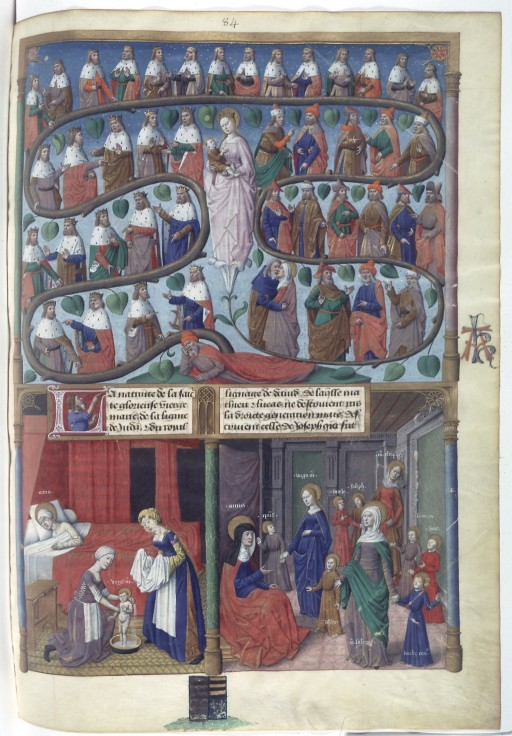
\includegraphics[height=30\baselineskip]{Tree_of_Jesse.jpeg}
\caption{Eine Darstellung des Baums Jesse,\footnote{Miniatur von Jacques de Besançon, Paris, etwa 1485, \url{https://commons.wikimedia.org/wiki/File:Bnf_Ms_Fran\%C3\%A7ais_245,_fol._84,_Arbre_de_Jess\%C3\%A9.jpg}} unten Geburt der Maria}
\end{center}
\end{figure}


\end{document}
